%%Berichtvorlage für EDBV WS 2014/2015

\documentclass[paper=A4, deutsch]{scrartcl}
\usepackage[ngerman]{babel}
\usepackage[utf8]{inputenc}
\usepackage{algorithmic}
\usepackage{algorithm}
\usepackage{graphicx}
\usepackage{amsmath,amssymb}
\usepackage{subcaption}
\captionsetup{compatibility=false}
\usepackage{multirow}
\usepackage{color}
\usepackage[]{geometry}


\begin{document}


%%------------------------------------------------------
%% Ab hier tragt ihr eure Daten und Ergebnisse ein:
%%------------------------------------------------------

\title{Schnapskönig} %%Projekttitel hier eintragen

\subtitle{EDBV WS 2017/2018: AG\_A2} %%statt XX Arbeitsgruppenbezeichnung hier eintragen (zB.: A1)


%%Namen und Matrikelnummern der Gruppenmitglieder hier eintragen
\author{Jan Michael Lajarno (01425799)\\
Andreas Brunner (01429369)\\
Miran Jank (01526438)\\
Thorsten Korpitsch (01529243)\\
Aleksandar Marinkovic (01634028)\\
}


%%------------------------------------------------------

\maketitle


%%------------------------------------------------------
\section{Gewählte Problemstellung}
\subsection{Ziel}
\textit{Beim Schnappsen treten 2 Spieler gegeneinander an. Zu Beginn bekommt jeder 5 Karten vom Stapel, danach wird jede Runde von beiden Spielern eine Karte gezogen. Jede Runde wird jeweils 1 Karte von jedem Spieler auf den Tisch gelegt wobei beide Spieler versuchen einen Stich zu machen.
Stechen bedeutet, dass die eigene Karte entweder ein Adut ist und die Karte des gegenübers keines ist, beziehungsweise, dass die eigene Karte einen höheren Wert hat als die des Gegenübers. Es wird solange gespielt bis der Stapel leer ist und beide Spieler keine Karten mehr auf der Hand haben, beziehungsweise
einer der Spieler Karten im Wert von 66 Punkten gestochen hat. Sind alle Karten ausgespielt worden, wird der Gewinner ermittelt indem die gewonnenen Punkte beider Spieler gezählt werden und danach der mit der höheren Punktezahl gewinnt.}
\subsection{Eingabe}
\textit{Der Benutzer muss pro Spielzug ein Farbbild, in einem gängigen Format(.PNG/.JPG/.JPEG), der Karten in das Programm laden.}
\subsection{Ausgabe}
\textit{In der Konsole wird ein Zwischenstand nach jeder Runde ausgegeben, am Ende wird der Gewinner ausgegeben und der Endstand.}
\subsection{Voraussetzungen und Bedingungen}
\textit{Ein Farbbild der Karten. Der Hintergrund sollte möglichst Einfarbig sein (nicht weiß, texturarm). Die Kamera soll sich in einem Winkel von 45 bis 135 Grad befinden. Die Karten müssen mit einem dünnen schwarzen Rand preperiert sein. Die obere Karte darf maximal 45\% der anderen Karte überdecken.}
\subsection{Methodik}
\begin{enumerate}
	\item Threshold nach Otsu: Um in Kombination mit Zusammenhangskomponenten die Karten zu trennen
	\item Geometrische Transformation: Um das Eingabebild vorzubereiten wird aus dem, bis zu 45 Grad schrägen Bild, ein Bild aus der Vogelperspektive (90 Grad) transformiert, die hochkant steht
	\item Template-Matching: Um die Spielkarte zu identifizieren 
\end{enumerate}
\subsection{Evaluierung}
\begin{itemize}
	\item Werden beide Karten erkannt?
	\item Wird das Bild richtig transformiert, oder werden Buchstaben/Symbole verzerrt?
	\item Wird die Karte richtig identifiziert?
\end{itemize}

\subsection{Datenbeispiel}
\begin{figure}[h!]
 \centering
 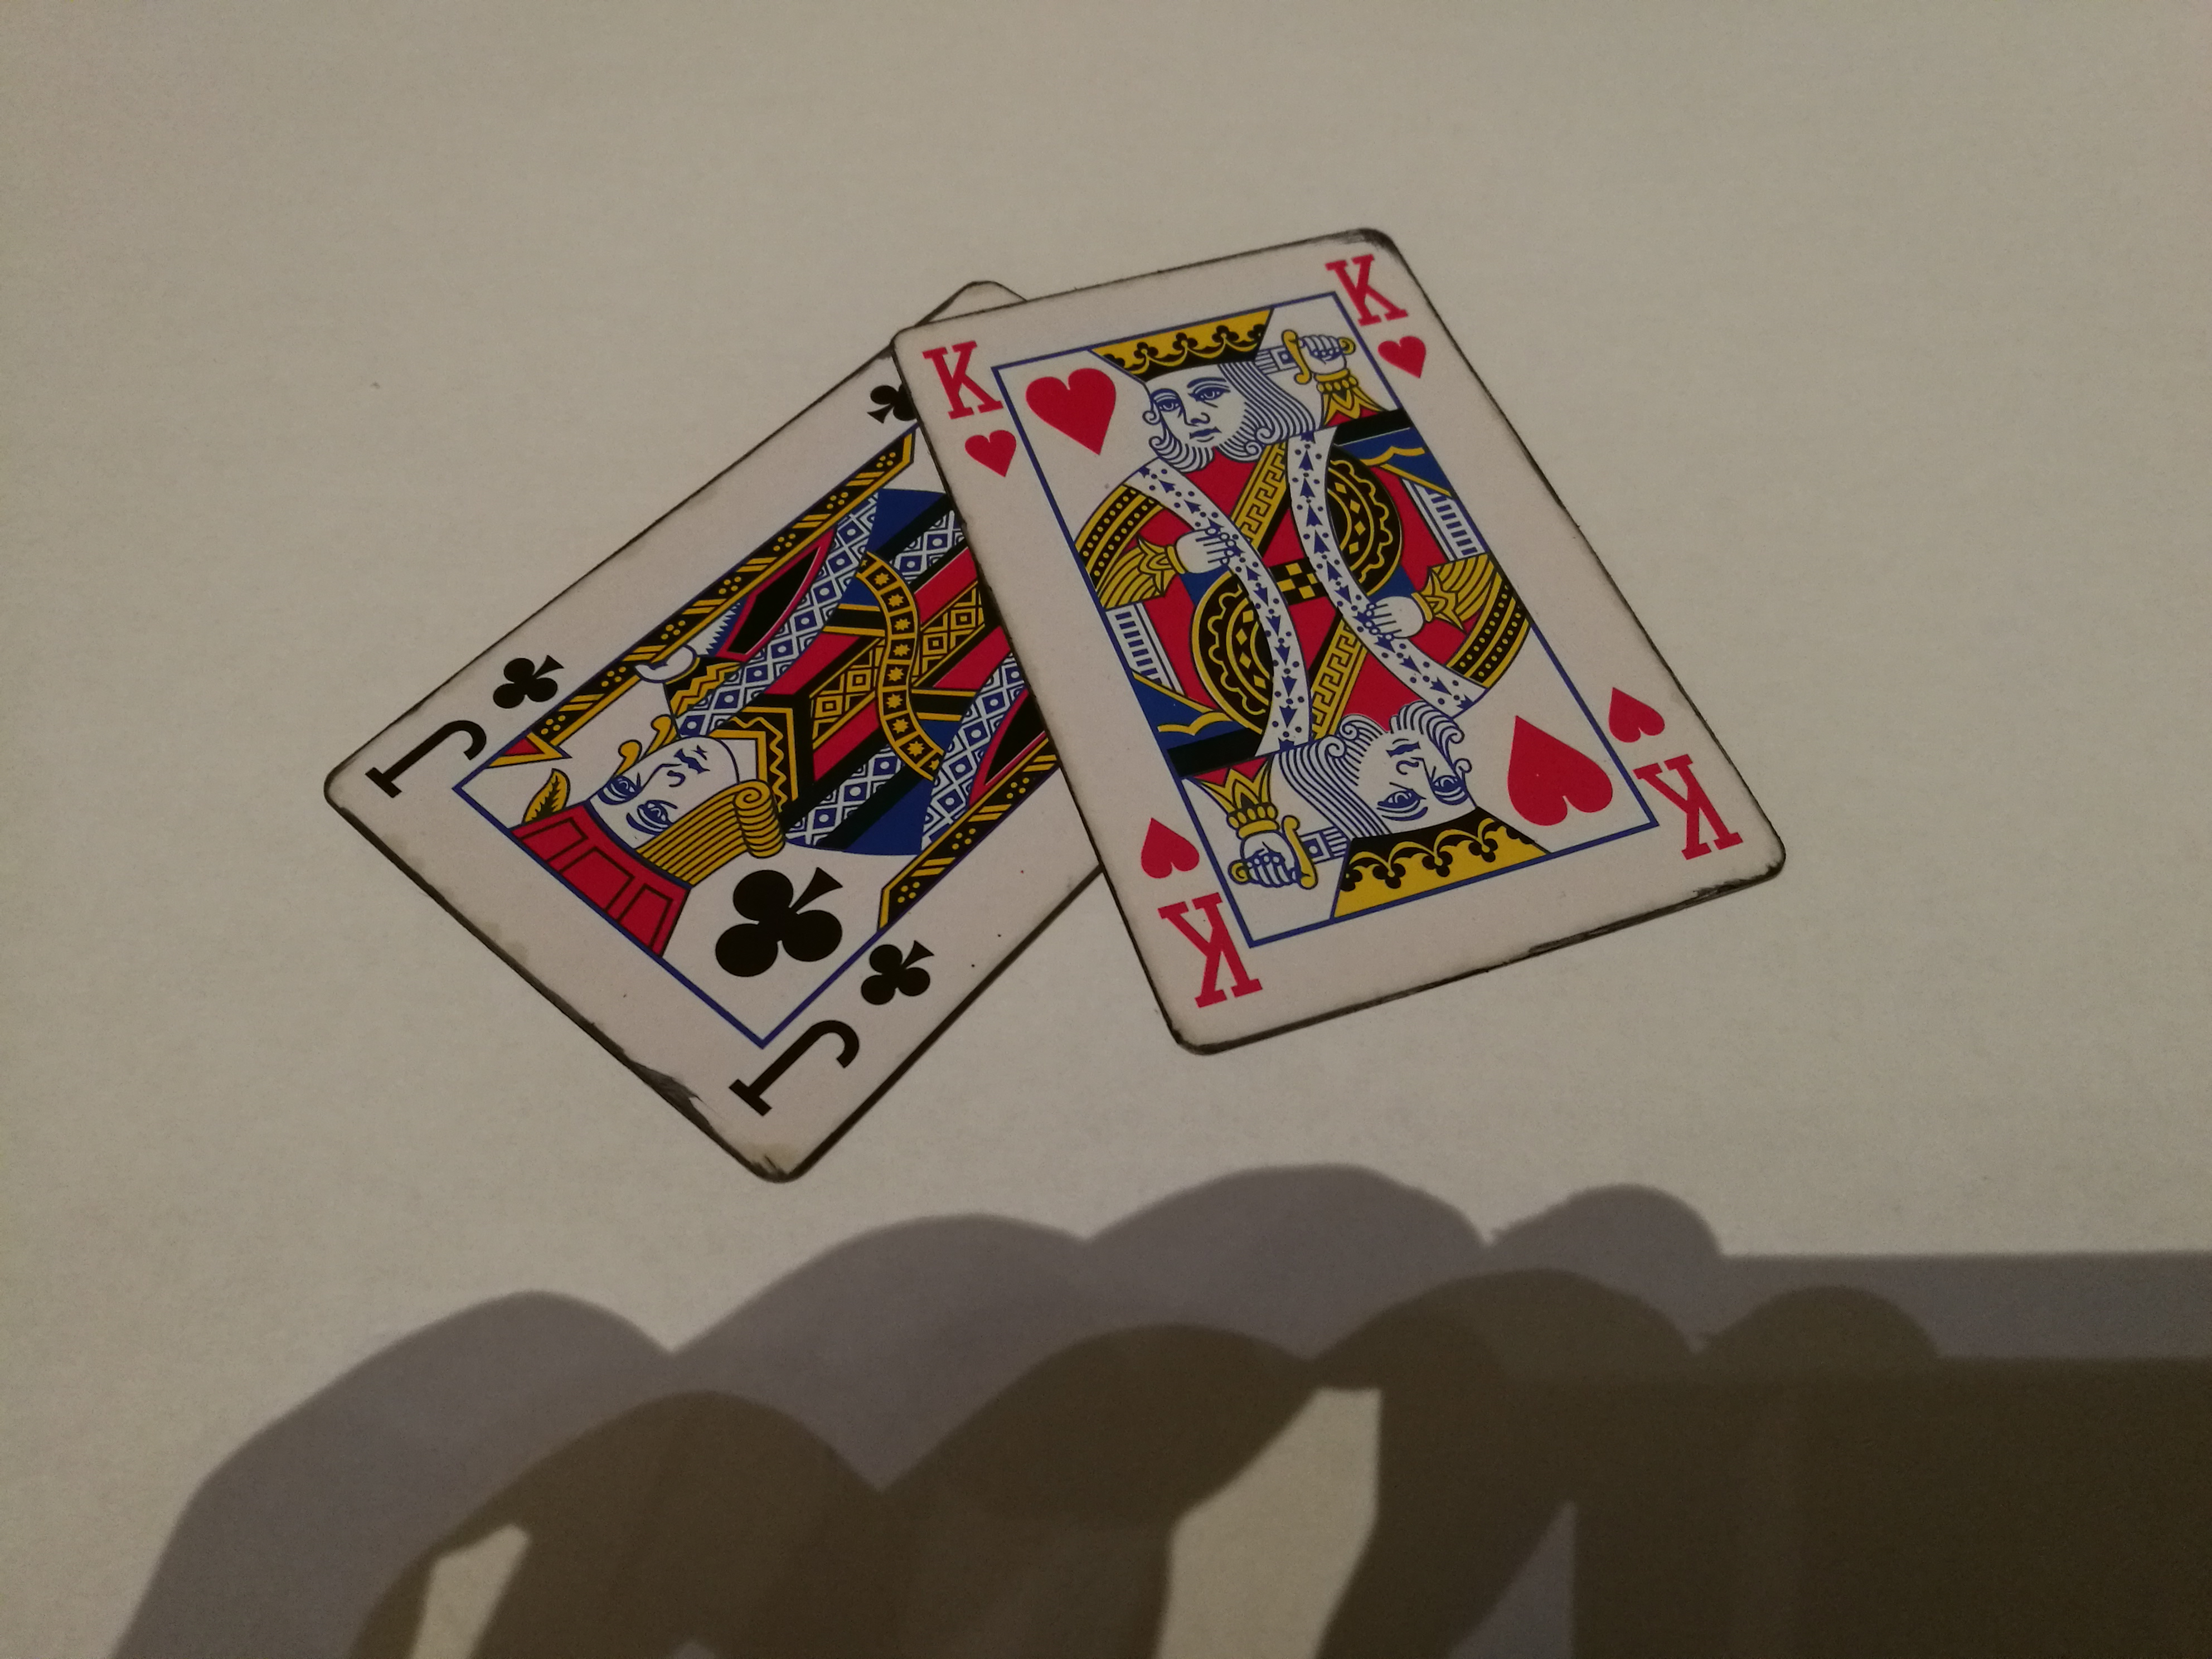
\includegraphics[width=0.5\textwidth]{datenbeispiel.jpg}
 \caption{Kreuz-Bube sticht Herz-König, 6 Punkte gewonnen}
 \label{fig:img}
\end{figure}
\begin{figure}[h!]
 \centering
 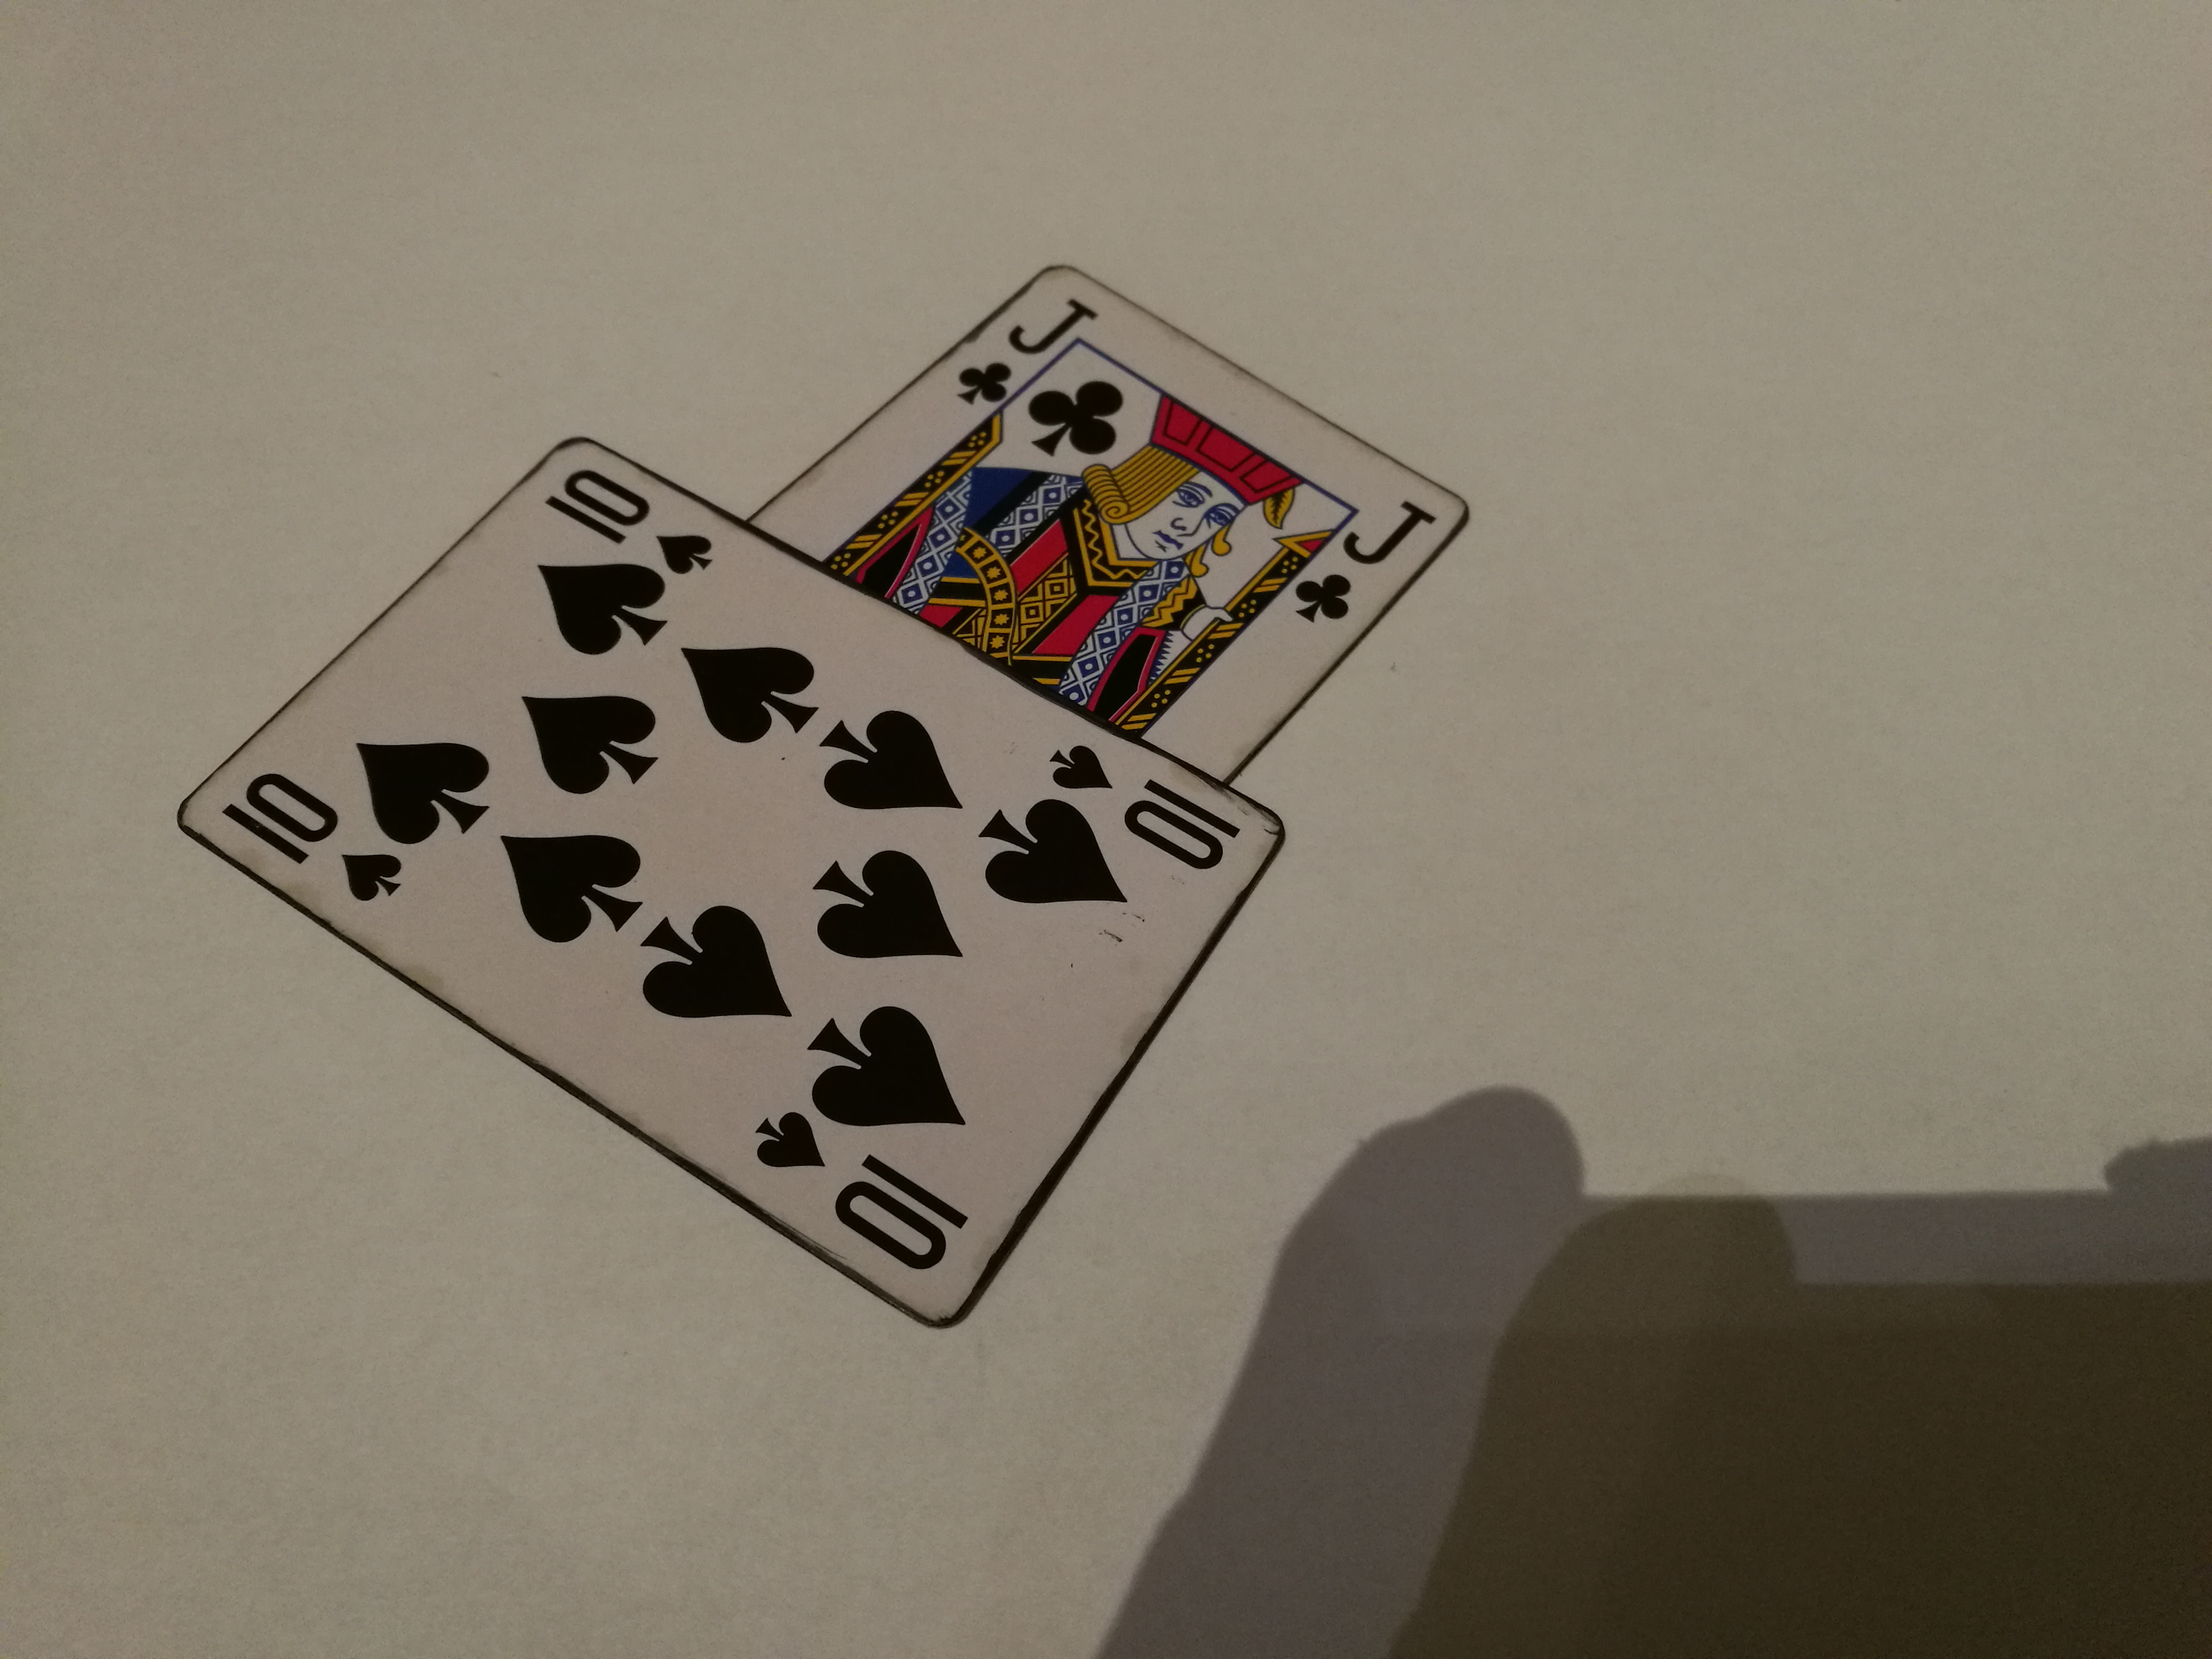
\includegraphics[width=0.5\textwidth]{datenbeispiel2.jpg}
 \caption{Kreuz-Bube sticht Pik-10, 12 Punkte gewonnen}
 \label{fig:img}
\end{figure}

\newpage

\subsection{Zeitplan}
\begin{table}[h!]
	\centering
		\begin{tabular}{|c|c|c|c|c|}
		\hline
		Meilenstein & \multicolumn{2}{c|}{abgeschlossen am} & \multicolumn{2}{c|}{Arbeitsaufwand in h}\\
		\cline{2-5}
		 & geplant & tatsächlich & geplant & tatsächlich\\
		\hline
		Vorarbeit Projekt& 20.10.2017 & 21.10.2017 & 20 & 23\\
		Prototyp erstellen& 10.11.2017& 01.12.2017 & 40 & 80\\
		Geometrische Transformation& 22.12.2017& 27.12.2017 & 105  & 92 \\
		Threshhold nach Otsu& 18.12.2017& 25.12.2017 & 67 & 60 \\
		Pattern-Matching & 18.12.2017 &30.12.2017 & 43 & 30\\
		GT-Test & 31.12.2017& 31.12.2017 & 10  & 12 \\
		TH-Test & 27.12.2017 & 29.12.2017 & 5 & 5 \\
		PM-Test & 27.12.2017& 29.12.2017 & 5 & 3 \\
		Unit-Test & 05.01.2017& 04.01.2017 & 5 & 2 \\
		\hline
		\end{tabular}
\end{table}
%%------------------------------------------------------

%%------------------------------------------------------

 \newpage

\section{Arbeitsteilung}
\begin{center}
  \begin{tabular}{ |l |p{0.7\linewidth} | }
    \hline
  Name & Tätigkeiten\\
    \hline
		Jan Michael Lajarno & Matlab: Prototyp, rotateCard, findEdges \newline Bericht: Gewählte Problemstellung\\
		\hline
		Andreas Brunner & Matlab: Prototyp, scaleCard, tmc \newline Bericht: Arbeitsteilung, Methodik(Template Matching)\\
		\hline
		Miran Jank & Matlab: Prototyp, GUI, geometricTransform \newline Bericht: Schlusswort, Titelseite, Methodik(Geometrische Transformation)\\
		\hline
		Thorsten Korpitsch & Matlab: Prototyp, ausführbares Programm, splitCards, thresholdOtsu \newline Bericht: Evaluierung, Methodik(Threshhold nach Otsu)\\
		\hline
		Aleksandar Marinkovic & Matlab: Prototyp, geometricTransform \newline Bericht: Methodik(Geometrische Transformation), Implementierung\\ 
		\hline
  \end{tabular}
\end{center}

%%------------------------------------------------------

%%------------------------------------------------------
\section{Methodik}
(2-3 Seiten)\\
Hier wird die verwendete Methodik in der Theorie vorgestellt:\\
Welche Methodik wurde verwendet? Warum eignet sich diese Methodik für die gewählte Problemstellung? Habt ihr Methoden verändert (Einschränkungen, Abwandlungen), wenn ja wie? etc.\\
Die erwähnten Methoden werden zum größten Teil auf Beschreibungen in Büchern oder wissenschaftlichen Artikeln beruhen. Daher ist hier auch der richtige Platz für Zitate. Die hier zitierten Publikationen sollten mittels Abkürzung bzw. Nummer referenziert sein und sich in der Referenzliste am Ende des Berichts über diese Bezeichnung finden lassen.\\
Ein Beispielsatz (inkl. entsprechender Literaturangabe am Ende des Berichts): Interest Points wurden mittels Scale Invariant Feature Transform detektiert.\\
Bei der Verwendung von Latex gestaltet sich das Zitieren besonders einfach - siehe Beispielssatz im Source der Latex-Vorlage.\\
\textbf{Wichtig in diesem Abschnitt ist, dass sich der Leser eures Berichts mit den verwendeten Methodiken auskennen und wissen, weshalb ihr diese Methodiken verwendet habt und keine anderen. Es soll dem Leser helfen den nächsten Abschnitt des Berichts besser zu verstehen.}
%%------------------------------------------------------

%%------------------------------------------------------
\section{Implementierung}
(1-X Seiten)\\
Hier gebt ihr einen Überblick über eure Implementierung:\\
Wie habt ihr die im vorhergehenden Abschnitt vorgestellte Methodik praktisch umgesetzt? Wie werden die einzelnen Methoden kombiniert (zB. Implementierungspipeline)?\\
Hier ist Platz für Implementierungsdetails wie zB. gewählte Parameter. \\
Wie startet der User das Programm? Welche Parameter hat der User zu setzen?\\
Auch in diesem Abschnitt können Referenzen und Zitate notwendig sein.\\
\textbf{Wichtig in diesem Abschnitt ist, dass der Leser eures Berichts versteht wie ihr euer Projekt in MATLAB umgesetzt habt um sich auch im Quelltext leichter zurechtfinden zu können.}
%%------------------------------------------------------

%%------------------------------------------------------
\section{Evaluierung}
(2-X Seiten)\\
Hier stellt ihr euren Datensatz vor und beantwortet Evaluierungsfragen:\\
z.B. Fakten zum Datensatz: Anzahl der Bilder, Größe der Bilder, Quelle des Datensatzes (falls selbst aufgenommen: Aufnahmegerät, Einstellungen,... / falls nicht selbst erstellt: Datenbank vostellen... $\to$ Referenzen!)\\
Diskussion der Evaluierungsfragen: Beantwortung der Fragen, Diskussion anhand von Beispielen, Diskussion von Grenzfällen: für welche Bilder funktioniert die Implementierung, für welche nicht? Worin unterscheiden sich diese Bilder? Warum funktionieren sie nicht? etc.\\
Evaluiert wird der ganze Datensatz, nicht nur einzelne Bilder. Einzelne Bilder können zum Aufzeigen von Fehlern/Problemen/besonders guten Ergebnissen... genutzt werden.\\
Zur Evaluierung gehört auch das Testen der einzelnen Methodiken (separat), mit Erwähnung eventueller Einschränkungen.
%%------------------------------------------------------

%%------------------------------------------------------
\section{Schlusswort}
(max. 1 Seite)\\
Hier fasst ihr Ergebnisse eures Projekt zusammen:\\
Welche Schlussfolgerung lässt sich ziehen? Gibt es offene Probleme? Wie lässt sich eure Lösung noch verbessern? etc.

%%------------------------------------------------------

%%------------------------------------------------------
\bibliographystyle{plain}
\bibliography{edbv_lit}
%%Bei verwendung von Latex schreibt ihr eure Referenzen in ein eigenes bib-File (siehe hier edbv_lit.bib). Jene Referenzen, die ihr im Bericht mittels \cite zitiert, werden automatisch in die Referenzliste übernommen. Weitere Information zum Einbinden von BibTex gibt es hier: http://www.bibtex.org/Using/de/
%%------------------------------------------------------

\end{document}
\grid
\grid
